\section{Simplification}

Two simplification functions are devised to reduce an input point set, either randomly or using a grid-based clustering approach.

Function \ccc{CGAL::random_simplify_point_set()} randomly deletes a user-specified fraction of points from the input point set. This algorithm is fast.

Function \ccc{CGAL::grid_simplify_point_set()} considers a regular grid covering the bounding box of the input point set, and clusters all points sharing the same cell of the grid by picking as representant one arbitrarily chosen point. This algorithm is slower than \ccc{CGAL::random_simplify_point_set()}.

\ccExample

The following example reads a point set and simplifies it by clustering.
\ccIncludeExampleCode{Point_set_processing_3/grid_simplification_example.cpp}

% Insert image grid_simplification.jpg/eps
\begin{center}
    % Image
    \begin{ccTexOnly}
        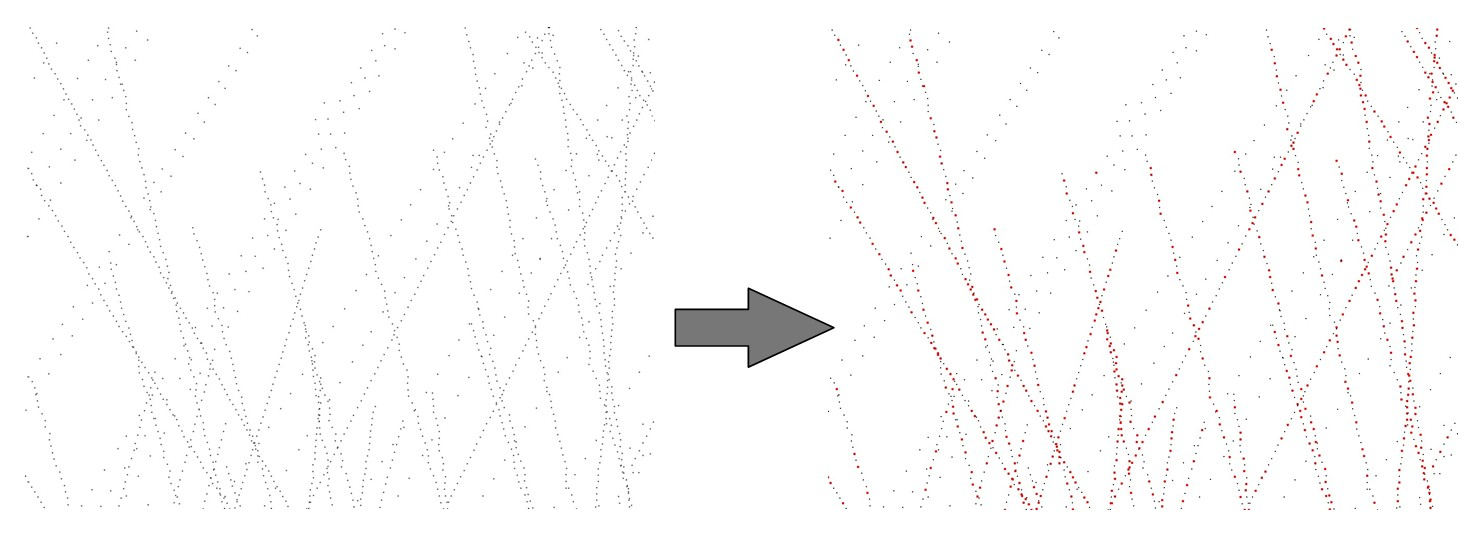
\includegraphics[width=1.0\textwidth]{Point_set_processing_3/grid_simplification} % omit .eps suffix
    \end{ccTexOnly}
    \begin{ccHtmlOnly}
        <img style="max-width: 100%;" border=0 src="../Point_set_processing_3/grid_simplification.jpg"><P>
    \end{ccHtmlOnly}
    % Title
    \begin{figure}[h]
        \caption{Point set simplification through grid-based clustering.
                 Removed points are depicted in red. Notice how
                 low-density areas (in green) are not simplified.}
        \label{Point_set_processing_3-fig-grid_simplification}
    \end{figure}
\end{center}



